% https://nrich.maths.org/problems/equivalent-pairs

% Tikz generating via claude.ai Sonnet 3.5

\documentclass{article}
\usepackage{tikz}
\begin{document}

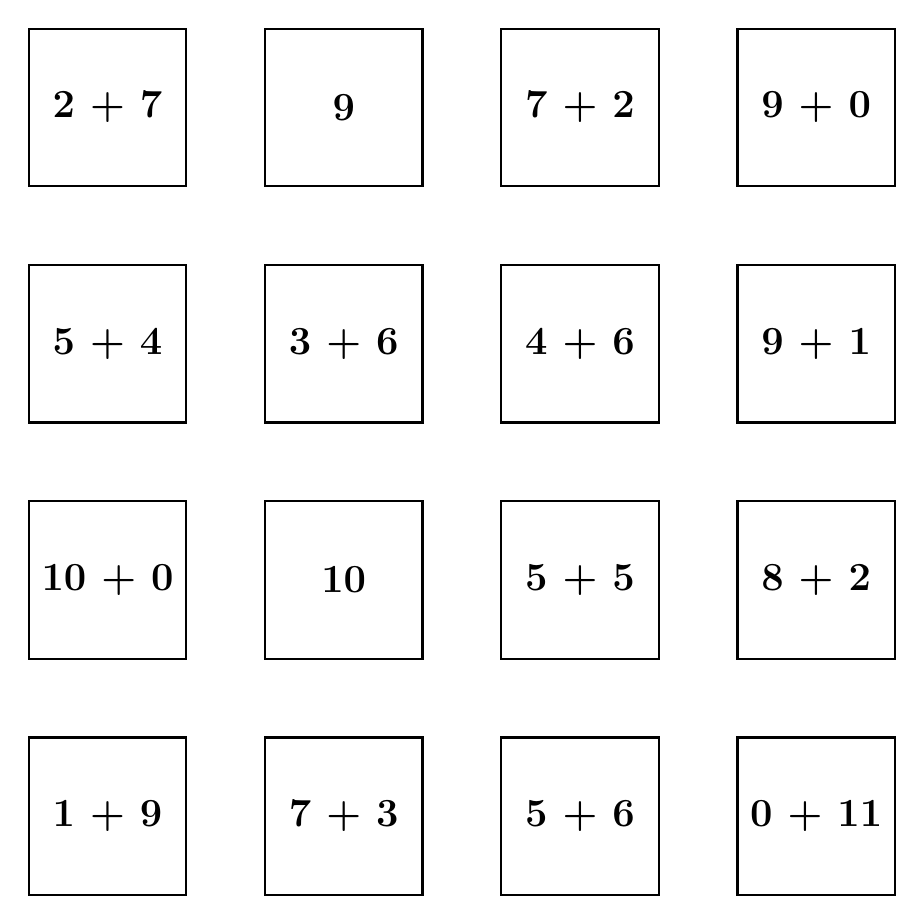
\begin{tikzpicture}[
    box/.style={
        draw,
        thick,
        minimum size=2cm,
        font=\Large\bfseries
    }
]

% First row
\node[box] at (0,0) {2 + 7};
\node[box] at (3,0) {9};
\node[box] at (6,0) {7 + 2};
\node[box] at (9,0) {9 + 0};

% Second row
\node[box] at (0,-3) {5 + 4};
\node[box] at (3,-3) {3 + 6};
\node[box] at (6,-3) {4 + 6};
\node[box] at (9,-3) {9 + 1};

% Third row
\node[box] at (0,-6) {10 + 0};
\node[box] at (3,-6) {10};
\node[box] at (6,-6) {5 + 5};
\node[box] at (9,-6) {8 + 2};

% Fourth row
\node[box] at (0,-9) {1 + 9};
\node[box] at (3,-9) {7 + 3};
\node[box] at (6,-9) {5 + 6};
\node[box] at (9,-9) {0 + 11};

\end{tikzpicture}

\end{document}